\documentclass[tikz]{standalone}
\usepackage[utf8]{inputenc}
\usepackage[T1]{fontenc}
\usepackage{amsmath, amssymb, graphicx, pgfplots, pifont, bm, bbm, booktabs, multicol, nicematrix}
\usetikzlibrary{shapes, graphs, shapes.geometric, decorations.pathmorphing, positioning, arrows, calc, arrows.meta, intersections, shadows.blur, patterns, patterns.meta}

\definecolor{testcolor}{RGB}{239,138,98}
\definecolor{traincolor}{RGB}{103,169,207}
\definecolor{ggplot2facetbg}{HTML}{E5E5E5}

\pagenumbering{gobble}

\begin{document}

% Model Evaluation 3CV
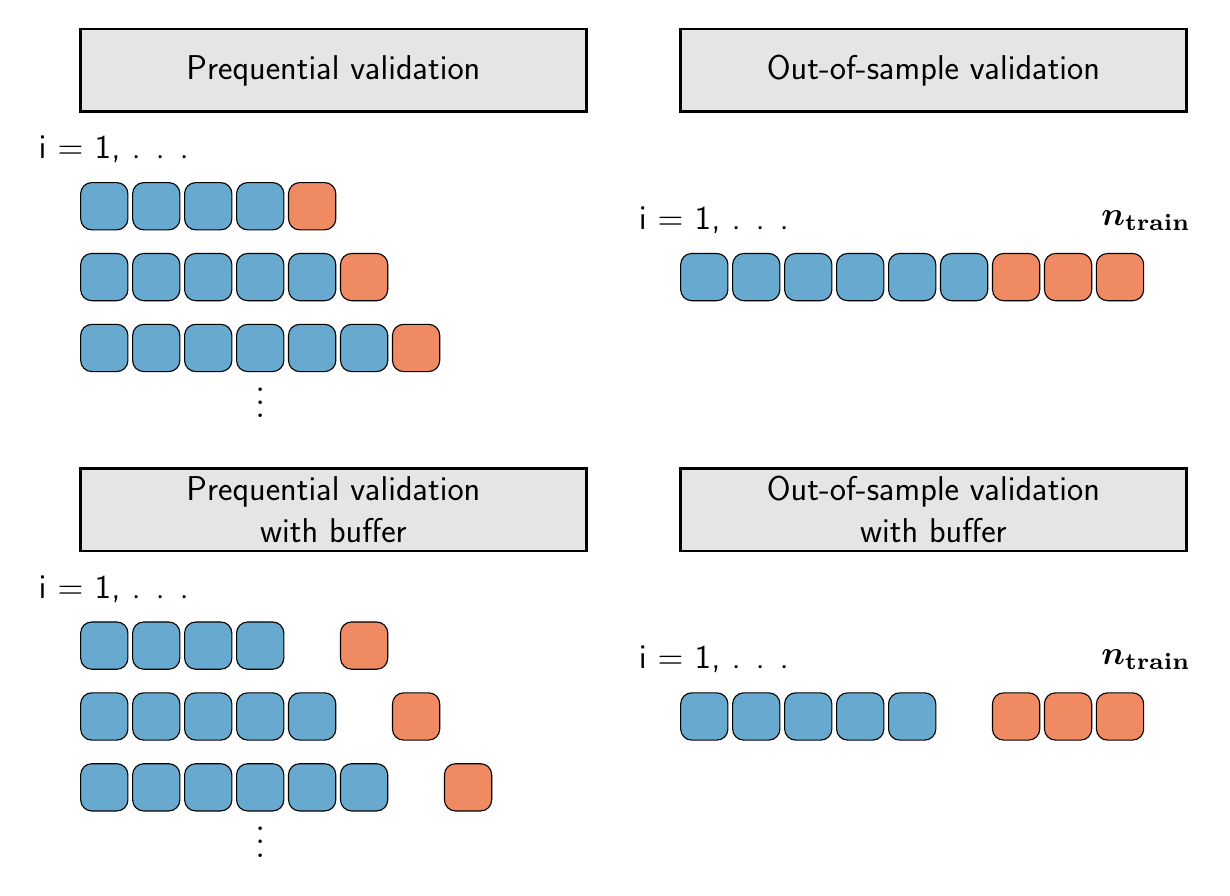
\begin{tikzpicture}[scale=0.6, every node/.style={transform shape}, shorten >=0.5pt, >={Stealth[round]}]

\def\x1{0}
\def\y1{0}

\draw[thick, fill = ggplot2facetbg, line width = 1, draw = black] (\x1, \y1 + 1 + 2 + 1.25) rectangle (\x1 + 8 + 0.7 + 1 + 1, \y1 + 1 + 0.5 + 1) node[pos=.5, font = \huge\sffamily, black, align=center] {Prequential validation};

% Insert the "i = 1, ..." text
\node[scale=2, font=\sffamily, black, align=center] at (\x1 + 0.7, \y1 + 1 + 0.7) {i = 1, . . .};

% boxes
\draw[fill = traincolor, draw = black, rounded corners] (\x1, \y1) rectangle +(1, 1) node[pos=.5, font = \huge] {};
\draw[fill = traincolor, draw = black, rounded corners] (\x1 + 1 + 0.1, \y1) rectangle +(1, 1) node[pos=.5, font = \huge] {};
\draw[fill = traincolor, draw = black, rounded corners] (\x1 + 2 + 0.2, \y1) rectangle +(1, 1) node[pos=.5, font = \huge] {};
\draw[fill = traincolor, draw = black, rounded corners] (\x1 + 3 + 0.3, \y1) rectangle +(1, 1) node[pos=.5, font = \huge] {};
\draw[fill = testcolor, draw = black, rounded corners] (\x1 + 4 + 0.4, \y1) rectangle +(1, 1) node[pos=.5, font = \huge] {};

\draw[fill = traincolor, draw = black, rounded corners] (\x1, \y1 - 1 - 0.5) rectangle +(1, 1) node[pos=.5, font = \huge] {};
\draw[fill = traincolor, draw = black, rounded corners] (\x1 + 1 + 0.1, \y1 - 1 - 0.5) rectangle +(1, 1) node[pos=.5, font = \huge] {};
\draw[fill = traincolor, draw = black, rounded corners] (\x1 + 2 + 0.2, \y1 - 1 - 0.5) rectangle +(1, 1) node[pos=.5, font = \huge] {};
\draw[fill = traincolor, draw = black, rounded corners] (\x1 + 3 + 0.3, \y1 - 1 - 0.5) rectangle +(1, 1) node[pos=.5, font = \huge] {};
\draw[fill = traincolor, draw = black, rounded corners] (\x1 + 4 + 0.4, \y1 - 1 - 0.5) rectangle +(1, 1) node[pos=.5, font = \huge] {};
\draw[fill = testcolor, draw = black, rounded corners] (\x1 + 5 + 0.5, \y1 - 1 - 0.5) rectangle +(1, 1) node[pos=.5, font = \huge] {};

\draw[fill = traincolor, draw = black, rounded corners] (\x1, \y1 - 2 - 2*0.5) rectangle +(1, 1) node[pos=.5, font = \huge] {};
\draw[fill = traincolor, draw = black, rounded corners] (\x1 + 1 + 0.1, \y1 - 2 - 2*0.5) rectangle +(1, 1) node[pos=.5, font = \huge] {};
\draw[fill = traincolor, draw = black, rounded corners] (\x1 + 2 + 0.2, \y1 - 2 - 2*0.5) rectangle +(1, 1) node[pos=.5, font = \huge] {};
\draw[fill = traincolor, draw = black, rounded corners] (\x1 + 3 + 0.3, \y1 - 2 - 2*0.5) rectangle +(1, 1) node[pos=.5, font = \huge] {};
\draw[fill = traincolor, draw = black, rounded corners] (\x1 + 4 + 0.4, \y1 - 2 - 2*0.5) rectangle +(1, 1) node[pos=.5, font = \huge] {};
\draw[fill = traincolor, draw = black, rounded corners] (\x1 + 5 + 0.5, \y1 - 2 - 2*0.5) rectangle +(1, 1) node[pos=.5, font = \huge] {};
\draw[fill = testcolor, draw = black, rounded corners] (\x1 + 6 + 0.6, \y1 - 2 - 2*0.5) rectangle +(1, 1) node[pos=.5, font = \huge] {};

% Vertical dots below the last row
\node[scale=2] at (\x1 + 3.5 + 0.3, \y1 - 2.2 - 2*0.5 - 0.25) {$\vdots$};

\def\x2{0}
\def\y2{-8.3}

\draw[thick, fill = ggplot2facetbg, line width = 1, draw = black] (\x2, \y2 + 2 + 1.25) rectangle (\x2 + 8 + 0.7 + 1 + 1, \y2 + 0.5 + 1) node[pos=.5, font = \huge\sffamily, black, align=center] {Prequential validation\\with buffer};

% Insert the "i = 1, ..." text
\node[scale=2, font=\sffamily, black, align=center] at (\x2 + 0.7, \y2 + 0.7) {i = 1, . . .};

% boxes
\draw[fill = traincolor, draw = black, rounded corners] (\x2, \y2 - 1) rectangle +(1, 1) node[pos=.5, font = \huge] {};
\draw[fill = traincolor, draw = black, rounded corners] (\x2 + 1 + 0.1, \y2 - 1) rectangle +(1, 1) node[pos=.5, font = \huge] {};
\draw[fill = traincolor, draw = black, rounded corners] (\x2 + 2 + 0.2, \y2 - 1) rectangle +(1, 1) node[pos=.5, font = \huge] {};
\draw[fill = traincolor, draw = black, rounded corners] (\x2 + 3 + 0.3, \y2 - 1) rectangle +(1, 1) node[pos=.5, font = \huge] {};
\draw[fill = testcolor, draw = black, rounded corners] (\x2 + 5 + 0.5, \y2 - 1) rectangle +(1, 1) node[pos=.5, font = \huge] {};

\draw[fill = traincolor, draw = black, rounded corners] (\x2, \y2 - 2 - 0.5) rectangle +(1, 1) node[pos=.5, font = \huge] {};
\draw[fill = traincolor, draw = black, rounded corners] (\x2 + 1 + 0.1, \y2 - 2 - 0.5) rectangle +(1, 1) node[pos=.5, font = \huge] {};
\draw[fill = traincolor, draw = black, rounded corners] (\x2 + 2 + 0.2, \y2 - 2 - 0.5) rectangle +(1, 1) node[pos=.5, font = \huge] {};
\draw[fill = traincolor, draw = black, rounded corners] (\x2 + 3 + 0.3, \y2 - 2 - 0.5) rectangle +(1, 1) node[pos=.5, font = \huge] {};
\draw[fill = traincolor, draw = black, rounded corners] (\x2 + 4 + 0.4, \y2 - 2 - 0.5) rectangle +(1, 1) node[pos=.5, font = \huge] {};
\draw[fill = testcolor, draw = black, rounded corners] (\x2 + 6 + 0.6, \y2 - 2 - 0.5) rectangle +(1, 1) node[pos=.5, font = \huge] {};

\draw[fill = traincolor, draw = black, rounded corners] (\x2, \y2 - 3 - 2*0.5) rectangle +(1, 1) node[pos=.5, font = \huge] {};
\draw[fill = traincolor, draw = black, rounded corners] (\x2 + 1 + 0.1, \y2 - 3 - 2*0.5) rectangle +(1, 1) node[pos=.5, font = \huge] {};
\draw[fill = traincolor, draw = black, rounded corners] (\x2 + 2 + 0.2, \y2 - 3 - 2*0.5) rectangle +(1, 1) node[pos=.5, font = \huge] {};
\draw[fill = traincolor, draw = black, rounded corners] (\x2 + 3 + 0.3, \y2 - 3 - 2*0.5) rectangle +(1, 1) node[pos=.5, font = \huge] {};
\draw[fill = traincolor, draw = black, rounded corners] (\x2 + 4 + 0.4, \y2 - 3 - 2*0.5) rectangle +(1, 1) node[pos=.5, font = \huge] {};
\draw[fill = traincolor, draw = black, rounded corners] (\x2 + 5 + 0.5, \y2 - 3 - 2*0.5) rectangle +(1, 1) node[pos=.5, font = \huge] {};
\draw[fill = testcolor, draw = black, rounded corners] (\x2 + 7 + 0.7, \y2 - 3 - 2*0.5) rectangle +(1, 1) node[pos=.5, font = \huge] {};

% Vertical dots below the last row
\node[scale=2] at (\x2 + 3.5 + 0.3, \y2 - 3.2 - 2*0.5 - 0.25) {$\vdots$};

\def\x3{12.7}
\def\y3{0}

\draw[thick, fill = ggplot2facetbg, line width = 1, draw = black] (\x3, \y3 + 1 + 2 + 1.25) rectangle (\x3 + 8 + 0.7 + 1 + 1, \y3 + 1 + 0.5 + 1) node[pos=.5, font = \huge\sffamily, black, align=center] {Out-of-sample validation};

% Insert the "i = 1, ..." text without the "n"
\node[scale=2, font=\sffamily, black, align=center] at (\x3 + 0.7, \y3 + 0.2) {i = 1, . . .};

% Insert the "n" text above the last box of color "testcolor"
\node[scale=2, font=\sffamily\boldmath, black] at (\x3 + 8 + 0.8 + 0.5 + 0.55, \y3 + 0.2) {$n_{\mathrm{train}}$};

% boxes
\draw[fill = traincolor, draw = black, rounded corners] (\x3, \y3 - 1 - 0.5) rectangle +(1, 1) node[pos=.5, font = \huge] {};
\draw[fill = traincolor, draw = black, rounded corners] (\x3 + 1 + 0.1, \y3 - 1 - 0.5) rectangle +(1, 1) node[pos=.5, font = \huge] {};
\draw[fill = traincolor, draw = black, rounded corners] (\x3 + 2 + 0.2, \y3 - 1 - 0.5) rectangle +(1, 1) node[pos=.5, font = \huge] {};
\draw[fill = traincolor, draw = black, rounded corners] (\x3 + 3 + 0.3, \y3 - 1 - 0.5) rectangle +(1, 1) node[pos=.5, font = \huge] {};
\draw[fill = traincolor, draw = black, rounded corners] (\x3 + 4 + 0.4, \y3 - 1 - 0.5) rectangle +(1, 1) node[pos=.5, font = \huge] {};
\draw[fill = traincolor, draw = black, rounded corners] (\x3 + 5 + 0.5, \y3 - 1 - 0.5) rectangle +(1, 1) node[pos=.5, font = \huge] {};
\draw[fill = testcolor, draw = black, rounded corners] (\x3 + 6 + 0.6, \y3 - 1 - 0.5) rectangle +(1, 1) node[pos=.5, font = \huge] {};
\draw[fill = testcolor, draw = black, rounded corners] (\x3 + 7 + 0.7, \y3 - 1 - 0.5) rectangle +(1, 1) node[pos=.5, font = \huge] {};
\draw[fill = testcolor, draw = black, rounded corners] (\x3 + 8 + 0.8, \y3 - 1 - 0.5) rectangle +(1, 1) node[pos=.5, font = \huge] {};

\def\x4{12.7}
\def\y4{-8.3}

\draw[thick, fill = ggplot2facetbg, line width = 1, draw = black] (\x4, \y4 + 2 + 1.25) rectangle (\x4 + 8 + 0.7 + 1 + 1, \y4 + 0.5 + 1) node[pos=.5, font = \huge\sffamily, black, align=center] {Out-of-sample validation\\with buffer};

% Insert the "i = 1, ..." text without the "n"
\node[scale=2, font=\sffamily, black, align=center] at (\x4 + 0.7, \y4 + 0.2 - 1) {i = 1, . . .};

% Insert the "n" text above the last box of color "testcolor"
\node[scale=2, font=\sffamily\boldmath, black] at (\x4 + 8 + 0.8 + 0.5 + 0.55, \y4 + 0.2 - 1) {$n_{\mathrm{train}}$};

% boxes
\draw[fill = traincolor, draw = black, rounded corners] (\x4, \y4 - 2 - 0.5) rectangle +(1, 1) node[pos=.5, font = \huge] {};
\draw[fill = traincolor, draw = black, rounded corners] (\x4 + 1 + 0.1, \y4 - 2 - 0.5) rectangle +(1, 1) node[pos=.5, font = \huge] {};
\draw[fill = traincolor, draw = black, rounded corners] (\x4 + 2 + 0.2, \y4 - 2 - 0.5) rectangle +(1, 1) node[pos=.5, font = \huge] {};
\draw[fill = traincolor, draw = black, rounded corners] (\x4 + 3 + 0.3, \y4 - 2 - 0.5) rectangle +(1, 1) node[pos=.5, font = \huge] {};
\draw[fill = traincolor, draw = black, rounded corners] (\x4 + 4 + 0.4, \y4 - 2 - 0.5) rectangle +(1, 1) node[pos=.5, font = \huge] {};
\draw[fill = testcolor, draw = black, rounded corners] (\x4 + 6 + 0.6, \y4 - 2 - 0.5) rectangle +(1, 1) node[pos=.5, font = \huge] {};
\draw[fill = testcolor, draw = black, rounded corners] (\x4 + 7 + 0.7, \y4 - 2 - 0.5) rectangle +(1, 1) node[pos=.5, font = \huge] {};
\draw[fill = testcolor, draw = black, rounded corners] (\x4 + 8 + 0.8, \y4 - 2 - 0.5) rectangle +(1, 1) node[pos=.5, font = \huge] {};

\end{tikzpicture}

\end{document}
